\section{Step 56 Publish the target and the replay boundary together}
Fill \texttt{seek\_publish}. Store the requested target at context offset 56 and the retained full-frame start at 64. Compute target minus start plus one with full-width arithmetic and store it at 72. Return success zero and active image count 16\,384. Retain all input fields and both suffix fields. The image copy precedes these stores; callers interpret the outputs only after the successful return. This is a single-threaded publication rule, not an atomic machine transaction for concurrent readers.

Use \texttt{s56-1} and stop before \texttt{seek\_published}.

\paragraph{Observe} At \texttt{seek\_published}, the ordinary example publishes target six, start four and replay count three. After return, repeat with extra-full: pixels match while start becomes five and replay count two. A later invalid target retains that actual successful image and all previously published outputs.

The replay count includes its starting full record. For target six, the ordinary
fixture applies records four, five and six: one full record followed by two deltas.
It does not apply six deltas from frame zero. In the extra-full control, record five
is also a full record, so the same target picture needs only records five and six.
The picture is unchanged by that representation choice; the published replay start
and count describe how this call obtained it.

For the bitmap observation, select the active destination at
\texttt{seek\_frame} plus four, beyond its leading guard. Use a custom display base,
512 by 512 display units and eight-unit pixels. Configure the entry-file header
before Debug so the display observes the complete destination copy. This path writes
every RGB word, so it does not require the initialized-picture option used for the
earlier one-pixel delta. Stop at \texttt{seek\_published}, then inspect the bitmap
and \texttt{seek\_context} in separate views.

Figure~\ref{fig:video-independent-seek} shows target six, replay start four and
count three. The first context pair retains scratch capacity; the next pairs publish
the target and replay boundary. Read each 64-bit value as a low/high pair of 32-bit
words in this little-endian run. The success return count is \texttt{0x4000} image
bytes, not the number of replayed records.

% Native editable composition from verified, unchanged IDE images.
\begin{figure}[htbp]
\centering
\sbox0{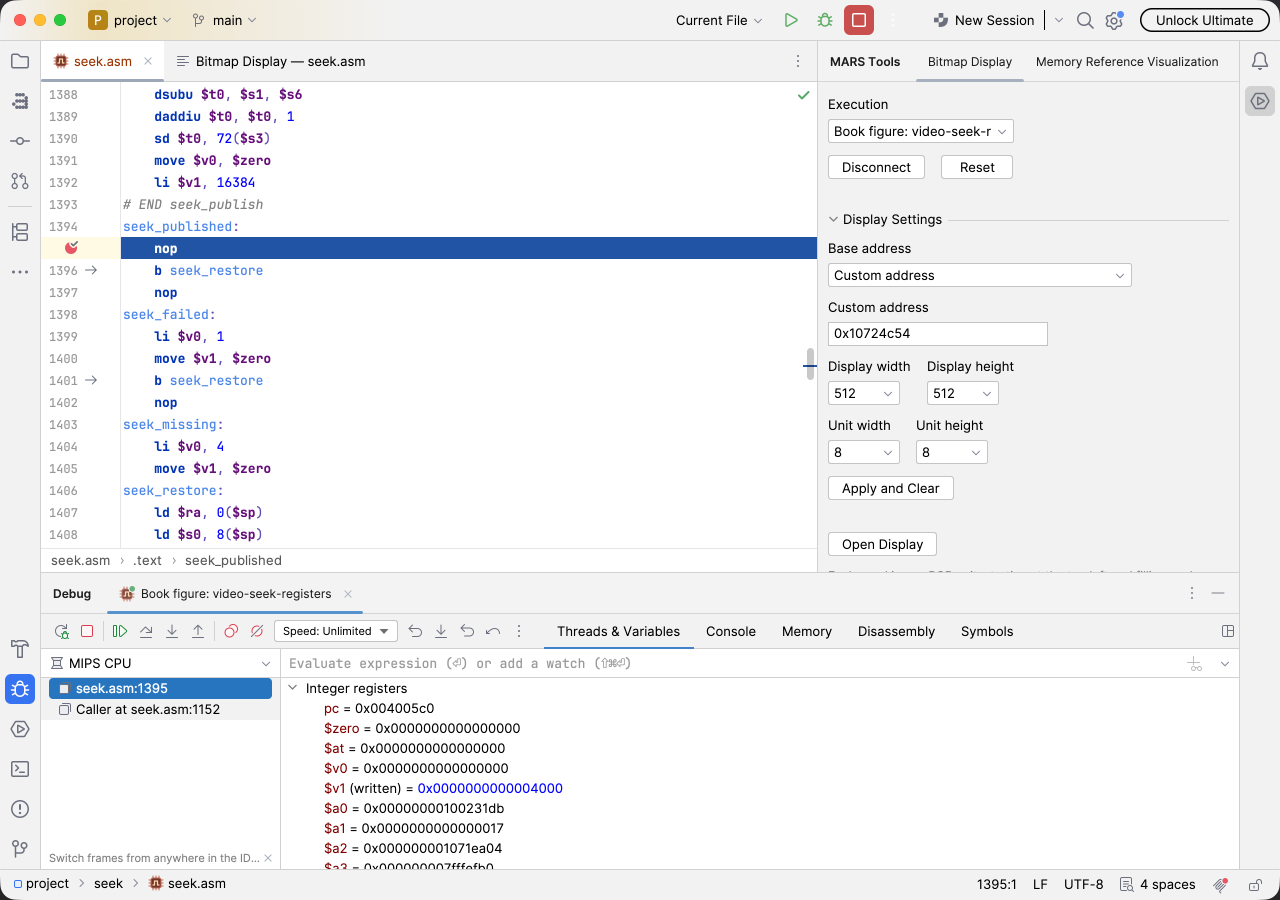
\includegraphics[artifact]{packages/034-lossless-video/captures/video-independent-seek/registers.png}}
\sbox2{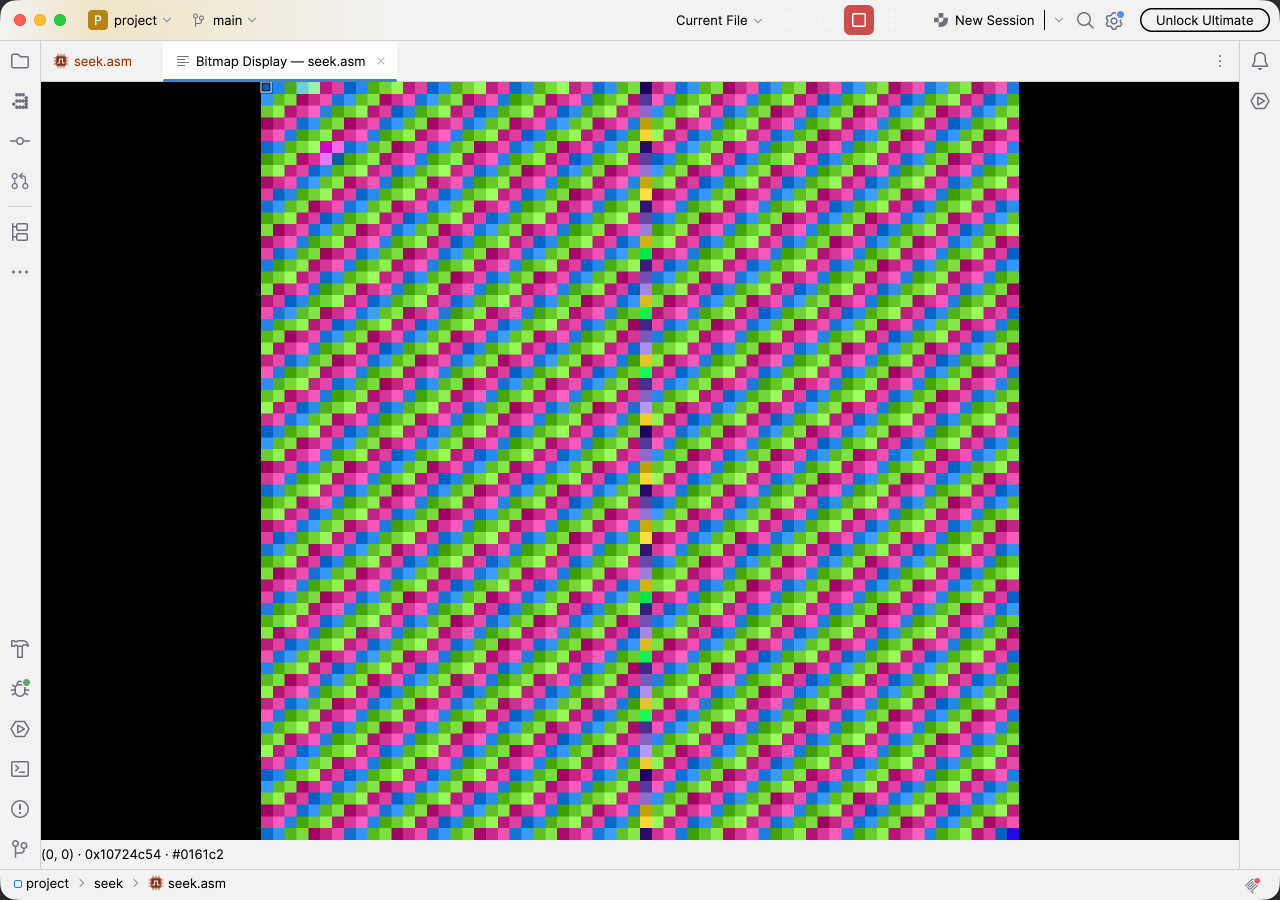
\includegraphics[artifact]{packages/034-lossless-video/captures/video-independent-seek/bitmap.png}}
\sbox4{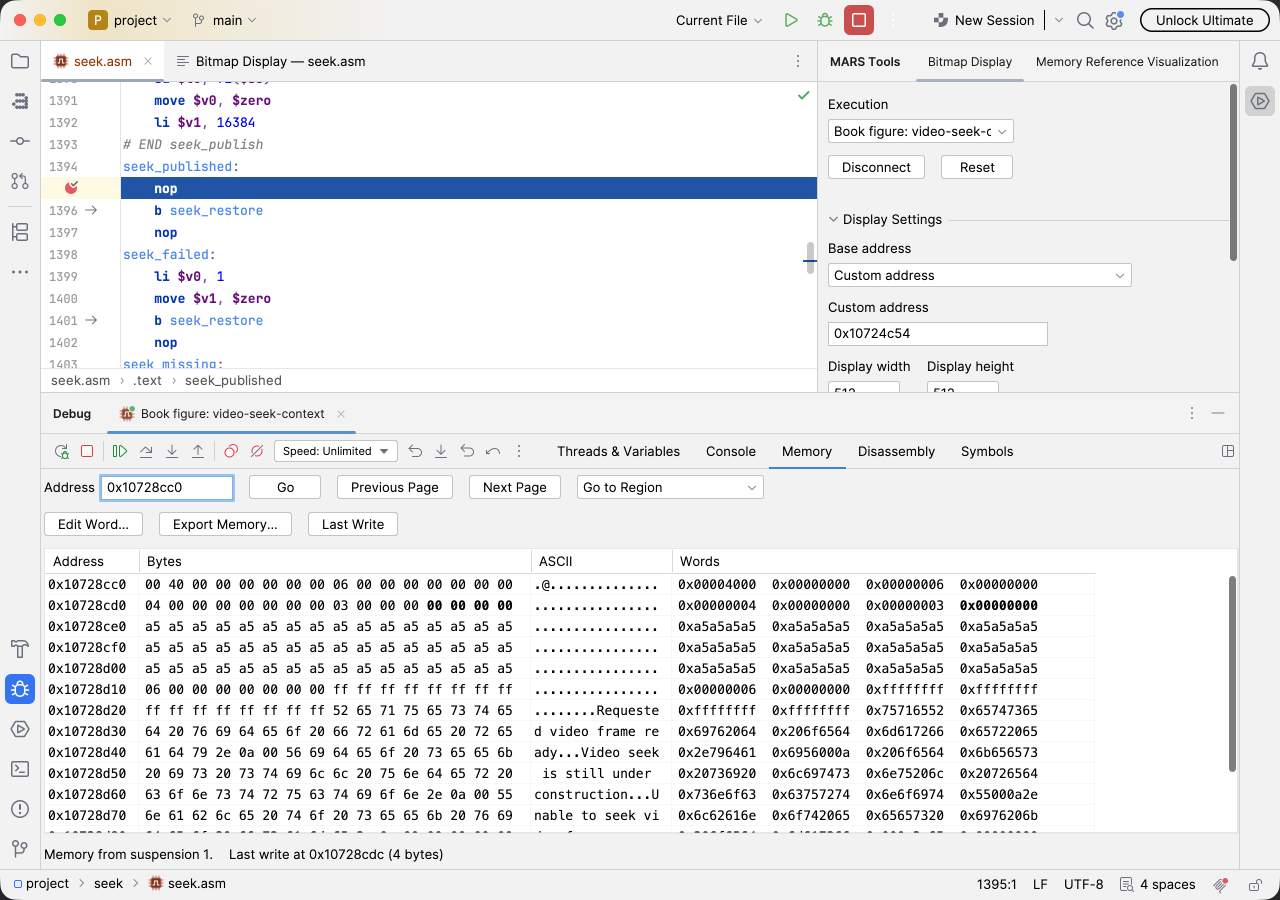
\includegraphics[artifact]{packages/034-lossless-video/captures/video-independent-seek/context.png}}
\edef\MARSseeksourceLeft{\the\dimexpr0.036718750\wd0\relax}
\edef\MARSseeksourceBottom{\the\dimexpr0.707777778\ht0\relax}
\edef\MARSseeksourceRight{\the\dimexpr0.611718750\wd0\relax}
\edef\MARSseeksourceTop{\the\dimexpr0.236666667\ht0\relax}
\edef\MARSseekbitmapLeft{\the\dimexpr0.199218750\wd2\relax}
\edef\MARSseekbitmapBottom{\the\dimexpr0.060000000\ht2\relax}
\edef\MARSseekbitmapRight{\the\dimexpr0.199218750\wd2\relax}
\edef\MARSseekbitmapTop{\the\dimexpr0.084444444\ht2\relax}
\edef\MARSseekcontextLeft{\the\dimexpr0.520312500\wd4\relax}
\edef\MARSseekcontextBottom{\the\dimexpr0.288888889\ht4\relax}
\edef\MARSseekcontextRight{\the\dimexpr0.139843750\wd4\relax}
\edef\MARSseekcontextTop{\the\dimexpr0.634444444\ht4\relax}
\edef\MARSseekreturnsLeft{\the\dimexpr0.246093750\wd0\relax}
\edef\MARSseekreturnsBottom{\the\dimexpr0.110000000\ht0\relax}
\edef\MARSseekreturnsRight{\the\dimexpr0.553906250\wd0\relax}
\edef\MARSseekreturnsTop{\the\dimexpr0.838888889\ht0\relax}
\begin{tikzpicture}[alt={Four annotated IDE details at seek_published. Detail 1 marks the next instruction. Detail 2 shows the reconstructed 64 by 64 target picture. Detail 3 shows little-endian low/high word pairs: scratch capacity 16384, target 6, full-frame replay start 4, replay count 3 and retained A5 suffix fields. Detail 4 shows success v0 equal to zero and v1 equal to 16384 image bytes.}]
\node[anchor=north west,inner sep=0,font=\small\bfseries] (source-title) at (6mm,0) {Paused seek publication};
\node[anchor=north west,inner sep=0] (source) at ([yshift=-1mm]source-title.south west) {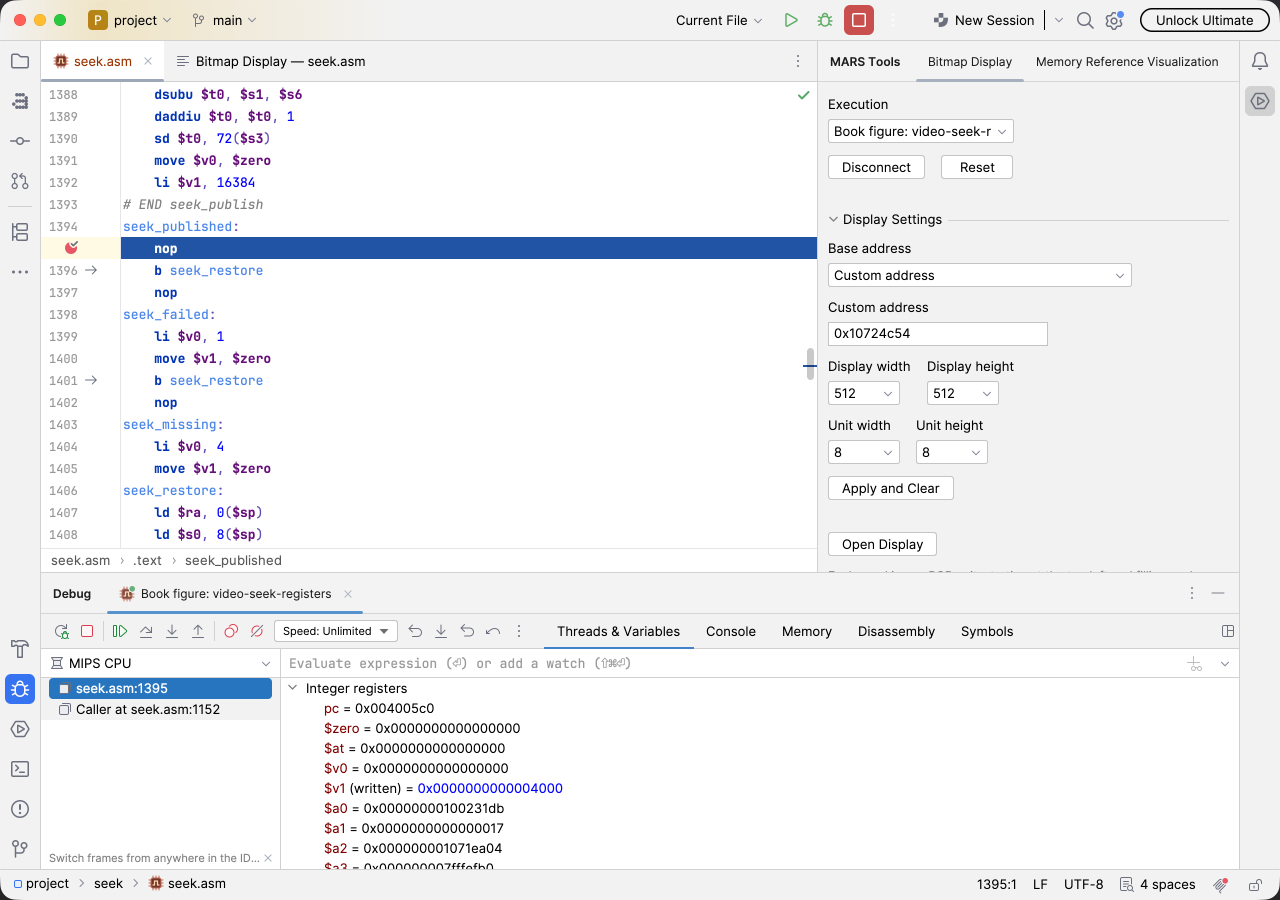
\includegraphics[width=0.66\linewidth,artifact,trim={\MARSseeksourceLeft{} \MARSseeksourceBottom{} \MARSseeksourceRight{} \MARSseeksourceTop{}},clip]{packages/034-lossless-video/captures/video-independent-seek/registers.png}};
\begin{scope}[shift={(source.south west)},x={($(source.south east)-(source.south west)$)},y={($(source.north west)-(source.south west)$)}]
\draw[black,line width=0.7pt] (0.168888889,0.080000000) rectangle (0.288888889,0.520000000);
\node[draw=black,fill=white,circle,inner sep=1.5pt,font=\footnotesize] at ($(0.168888889,0.520000000)+(-3mm,0)$) {1};
\end{scope}
\node[anchor=north west,inner sep=0,font=\small\bfseries] (bitmap-title) at ([yshift=-3mm]source.south west) {Independently reconstructed frame six};
\node[anchor=north west,inner sep=0] (bitmap) at ([yshift=-1mm]bitmap-title.south west) {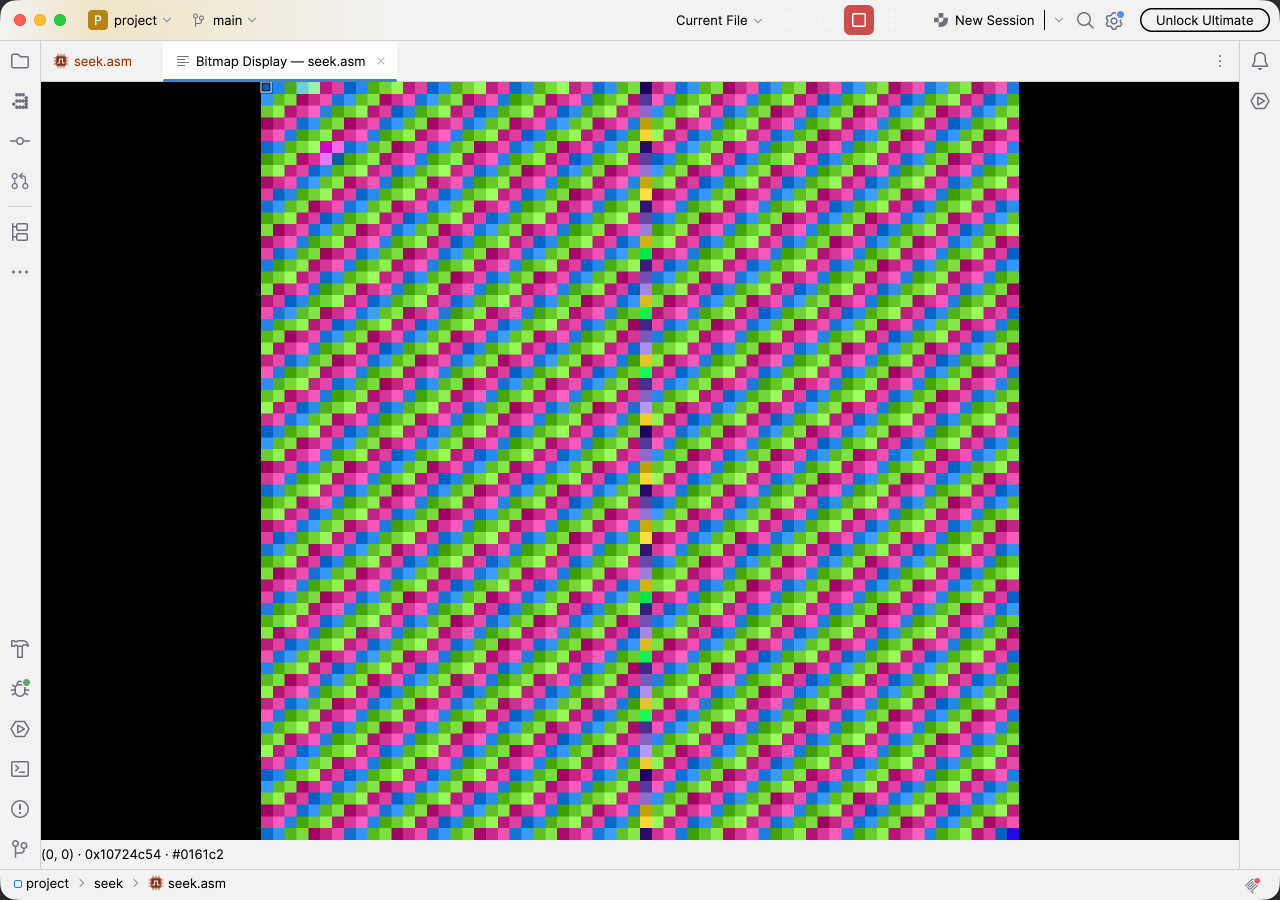
\includegraphics[width=0.47\linewidth,artifact,trim={\MARSseekbitmapLeft{} \MARSseekbitmapBottom{} \MARSseekbitmapRight{} \MARSseekbitmapTop{}},clip]{packages/034-lossless-video/captures/video-independent-seek/bitmap.png}};
\begin{scope}[shift={(bitmap.south west)},x={($(bitmap.south east)-(bitmap.south west)$)},y={($(bitmap.north west)-(bitmap.south west)$)}]
\draw[black,line width=0.7pt] (0.007792208,0.007792208) rectangle (0.992207792,0.992207792);
\node[draw=black,fill=white,circle,inner sep=1.5pt,font=\footnotesize] at ($(0.007792208,0.992207792)+(-3mm,0)$) {2};
\end{scope}
\node[anchor=north west,inner sep=0,font=\small\bfseries] (context-title) at ([yshift=-3mm]bitmap.south west) {Target and replay boundary in the context};
\node[anchor=north west,inner sep=0] (context) at ([yshift=-1mm]context-title.south west) {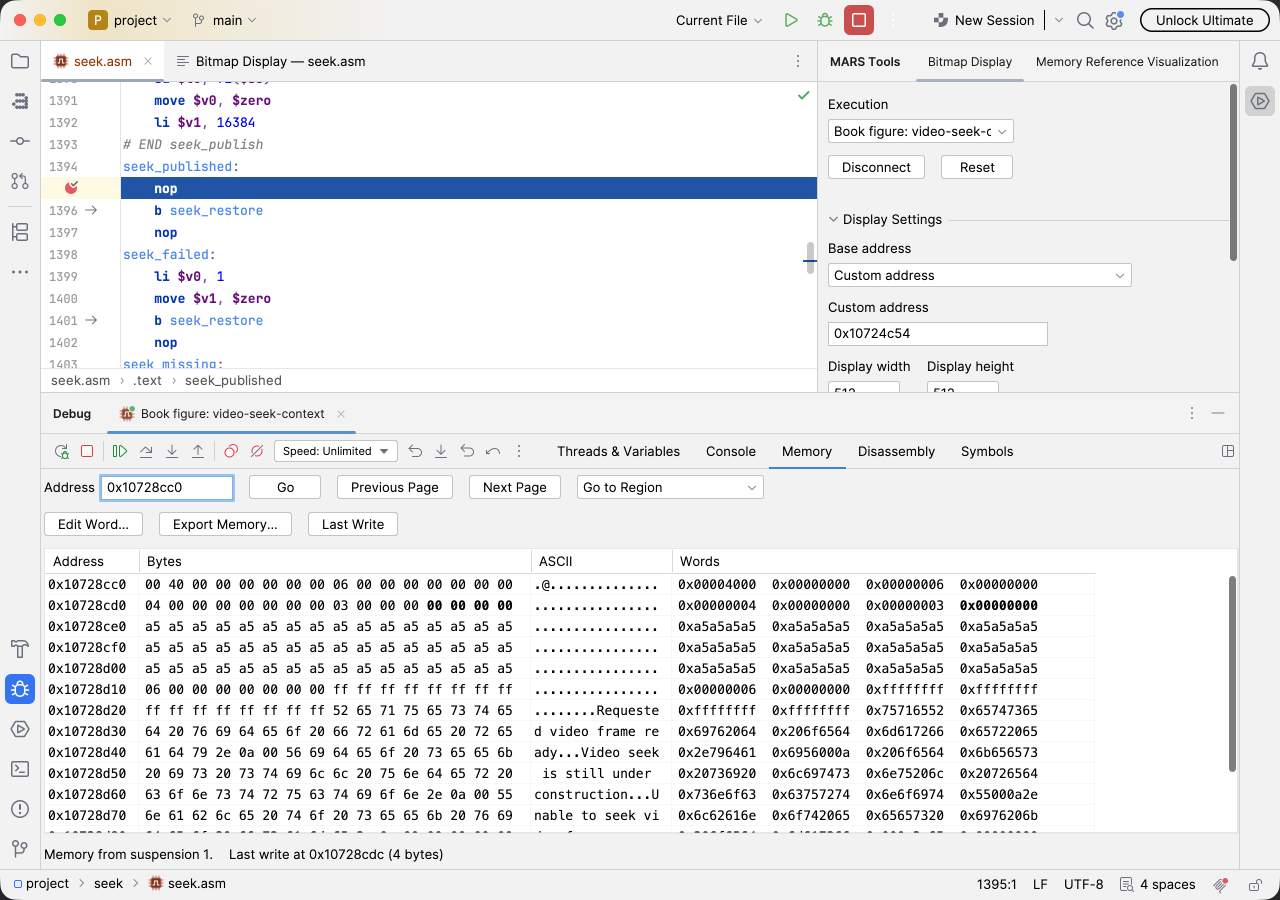
\includegraphics[width=0.74\linewidth,artifact,trim={\MARSseekcontextLeft{} \MARSseekcontextBottom{} \MARSseekcontextRight{} \MARSseekcontextTop{}},clip]{packages/034-lossless-video/captures/video-independent-seek/context.png}};
\begin{scope}[shift={(context.south west)},x={($(context.south east)-(context.south west)$)},y={($(context.north west)-(context.south west)$)}]
\draw[black,line width=0.7pt] (0.013793103,0.043478261) rectangle (0.986206897,0.956521739);
\node[draw=black,fill=white,circle,inner sep=1.5pt,font=\footnotesize] at ($(0.013793103,0.956521739)+(-3mm,0)$) {3};
\end{scope}
\node[anchor=north west,inner sep=0,font=\small\bfseries] (returns-title) at ([yshift=-3mm]context.south west) {Success and active image size};
\node[anchor=north west,inner sep=0] (returns) at ([yshift=-1mm]returns-title.south west) {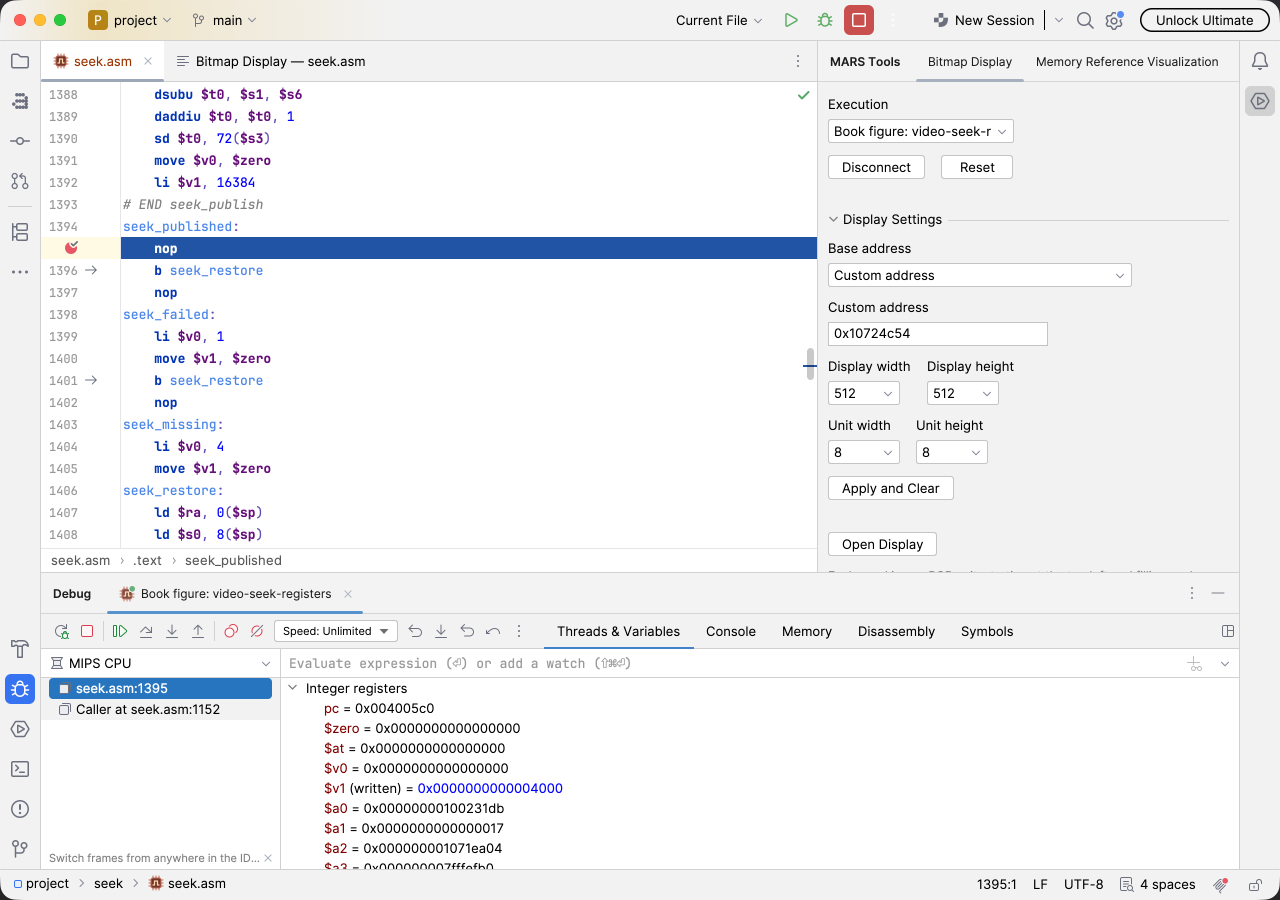
\includegraphics[width=0.5\linewidth,artifact,trim={\MARSseekreturnsLeft{} \MARSseekreturnsBottom{} \MARSseekreturnsRight{} \MARSseekreturnsTop{}},clip]{packages/034-lossless-video/captures/video-independent-seek/registers.png}};
\begin{scope}[shift={(returns.south west)},x={($(returns.south east)-(returns.south west)$)},y={($(returns.north west)-(returns.south west)$)}]
\draw[black,line width=0.7pt] (0.023437500,0.065217391) rectangle (0.976562500,0.934782609);
\node[draw=black,fill=white,circle,inner sep=1.5pt,font=\footnotesize] at ($(0.023437500,0.934782609)+(-3mm,0)$) {4};
\end{scope}
\end{tikzpicture}
\par\smallskip
\begin{minipage}{\linewidth}
\small
\begin{enumerate}
\item The checkpoint \texttt{nop} has not executed; the requested image and its context outputs have been published.
\item The complete picture was reconstructed into scratch and copied to the destination. It does not depend on a previously displayed frame.
\item Low/high pairs show retained scratch capacity \texttt{0x4000}, target six, replay start four and count three. The final \texttt{a5a5a5a5} pairs remain unchanged.
\item \texttt{\$v0} is zero; \texttt{\$v1} is \texttt{0x4000}, the 16\,384 bytes in 4096 RGB words.
\end{enumerate}
\end{minipage}
\caption{An independent seek to frame six. Three Debug launches show the same source, input and publication checkpoint.}
\label{fig:video-independent-seek}
\end{figure}

\clearpage

\paragraph{Check} What does the replay count measure?
\begin{enumerate}[label=\Alph*.]
  \item Milliseconds of playback.
  \item Applied records, including the starting full frame.
  \item All directory entries in the file.
\end{enumerate}
